\vspace{40px}\section{Bit Error Rate plot}
Another type of analysis that is important to make for the Hamming Code is its overall advantages during the transmission. Particularly, it is important to make a comparison between an encoded transmission (with error correction) and a not encoded transmission. To do so it is important to plot an important graph describing the relationship between the BER in relationship with the SNR value.

To plot such a graph it is necessary to evaluate the Bit Error Rate of the transmission of a random binary sequence with the given modulation (BPSK) for different Signal-to-Noise Ratio. The first thing to do is generate the random sequence and generate the BPSK carrier signal using the given \hyperref[initial-parameters]{initial parameters}:

\begin{lstlisting}
    % Initialize SNR vector
    SNR_vector = 0 : 1/2 : 15; 
        
    % Generation of binary sequence
    N = 1e4; % number of bits to be sent
    N = floor(N / k) * k; % match information block size
    binary_sequence = randi(2, 1, N) - 1;
    
    % Generate carrier signal
    
    % Define the time-step
    delta_t = tau / samples_per_symbol;
    
    % Time intervals for one symbol
    time_intervals = 0: delta_t: tau - delta_t;
    
    % Create the carrier signal
    carrier_signal = sin(2 * pi * f0 * time_intervals); % Carrier signal
    
    % Calculate the energy per symbol
    Eb = dot(carrier_signal, carrier_signal);
\end{lstlisting}

\noindent After creating the carrier signal it is necessary to encode and modulate the randomly generated sequence. To perform the Hamming encoding algorithm it is necessary to create a matrix that will be used in the algorithm. The functioning of the encoding is carefully explained in chapter \ref{hamming-encoding}. After Hamming-encoding the sequence the BPSK modulation is performed by transforming the sequence into a Non-Return-to-Zero signal and performing the \textit{Kronecke} multiplication with the carrier signal.

\begin{lstlisting}
    % Hamming encoding
    % Create the matrix for the Hamming-encoding algorithm
    binary_matrix = reshape(binary_sequence, k, N / k)';

    % Hamming-encode the matrix
    hamming_encoded_matrix = hamming_encoding(binary_matrix, codeword_length, k, generation_polynomial); % encode data
    hamming_encoded_matrix = hamming_encoded_matrix';

    % Unwrap the matrix into a single row
    hamming_encoded_sequence = hamming_encoded_matrix(:)';

    % Update the number of bits
    M = N;
    N = length(hamming_encoded_sequence);

    % Modulate the sequence with BPSK
    BPSK_signal = kron(-2 * hamming_encoded_sequence + 1, carrier_signal);
\end{lstlisting}

\noindent Before calculating the different BER values it is necessary to generate the noise power and standard deviation as follows:

\begin{lstlisting}
    % Generate noise power

    % Reversed SNR formula
    EbN0 = 10.^(SNR_vector / 10);
    
    % Obtain noise spectral power density
    N0 = Eb./EbN0;
    
    % Calculate sigma for BPSK
    sigma = sqrt(N0 / 2);  
    
    
    % Prepare the vectors for the for-loop
    BER_no_hamming = 1 : length(SNR_vector);
    BER_with_hamming = 1 : length(SNR_vector);
\end{lstlisting}

\noindent The crucial section of the analysis is presented in the following \texttt{for} loop. First of all the Gaussian White Noise is generated for every entry of the \texttt{SNR\_vector} variable and then added to the BPSK modulated signal. At this point, the detection is performed using the \href{https://github.com/imAlessas/telecom-lab-works/blob/main/reports/lab-4/Trigolo_Report_Lab4.pdf}{\textsl{optimal correlation receiver}} and the BPSK threshold which is zero. Before performing the error correction, the detected sequence is compared with the initial sequence to keep calculating the Bit Error Rate without performing the decoding (\texttt{BER\_no\_hamming}). Secondly, the error correction is performed using the detection algorithm, thoughtfully explained in chapter \ref{hamming-decoding}, and then the second BER value is computed (\texttt{BER\_with\_hamming}).

\begin{lstlisting}
    for i = 1 : length(SNR_vector)
        % Calculate the GWN for a specific SNR value
        noise = sigma(i) * randn(1, N * samples_per_symbol);

        % Add the noise
        signal_with_noise = BPSK_signal + noise; % add noise in transmitted channel;


        % Use CORRELATION RECEIVER to detect symbols

        % Slice recieved signal into segments in each column
        sliced_signal_with_noise = reshape(signal_with_noise, samples_per_symbol, N);

        % Detect the signal with the BPSK threshold
        detected_signal = carrier_signal * sliced_signal_with_noise < 0;

        
        errors_number_no_hamming = sum(detected_signal ~= hamming_encoded_sequence);

        % Calculate BER value
        BER_no_hamming(i) = errors_number_no_hamming / N;
        

        % Reshape the sequence into a matrix, every row is a codeword
        detected_sequence_matrix = reshape(detected_signal, codeword_length, N/codeword_length)';
        
        % Perform Hamming decoding
        decoded_data_matrix = hamming_decoding(detected_sequence_matrix, codeword_length, k, generation_polynomial); % encode data
        decoded_data_matrix = decoded_data_matrix';

        % Unwrap the matrix into a sequence
        decoded_data_sequence = decoded_data_matrix(:)'; 

        % Check number of erros
        errors_number_with_hamming = sum (decoded_data_sequence ~= binary_sequence);

        % Calculate BER value
        BER_with_hamming(i) = errors_number_with_hamming/M;
    end
\end{lstlisting}

\noindent All the information to plot the BER curve is known. The following script will provide the plots needed to properly analyze the impact of the cyclic Hamming coding during the noisy transmission. Noticeably, the BER graphics are not linear but should be plotted with the logarithmic scale.

\begin{lstlisting}
    % creates figure and settings
    f = figure(1);
    f.Name = 'Analysis of BER curve';
    f.NumberTitle = 'off';
    f.Position = [450, 100, 700, 600];
    
    % Draw plot without Hamming code
    semilogy(SNR_vector, BER_no_hamming, 'b'), grid on;

    % Draw plot with Hamming code
    hold on, semilogy(SNR_vector, BER_with_hamming, 'r'), hold off;

    % Draw theoretical plot
    hold on, semilogy(SNR_vector, error_propability, 'm'), hold off;

    % Draw SNR project value
    hold on, plot([SNR SNR], [1e-4, 1e-1], 'g--'), hold off;

    
    xlabel('Signal-to-Noise Ratio, [dB]'), ylabel('Bit Error Rate'); % lables
    ylim([1e-4, 1e-1]), xlim([0, 10]); % limits
    legend('Uncoded', 'Coded', 'Theoretical', 'Given SNR value'); % legend
\end{lstlisting}

\noindent By running the MATLAB script the plot obtained is displayed in figure \ref{fig:BER-plot}. As expected the red plot decreases faster than the blue plot. This is a reasonable and expected result because the error correction code decreases the error rate by correcting the errors occurring during the transmission. Additionally, the given SNR value is plotted with a dotted green line: the red and the green curves do not meet meaning that the given SNR value, the given modulation technique and the given channel coding algorithm are acceptable and valid to successfully perform a digital transmission. 

\begin{figure}[h]
    \centering
    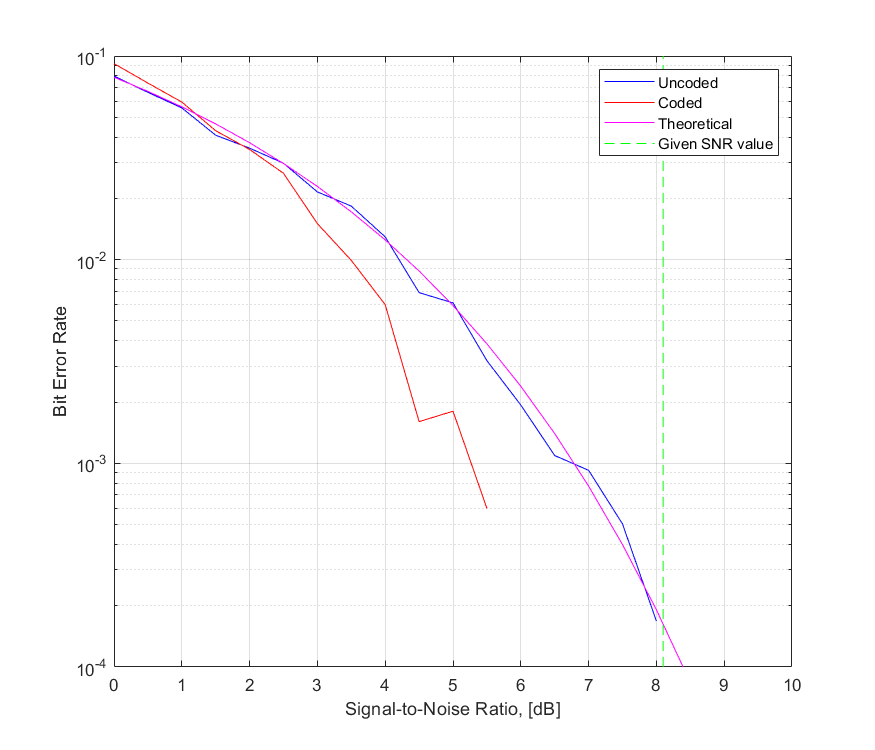
\includegraphics[width = \textwidth]{../res/imgs/BER-plot.png}
    \caption{BER vs SNR plot of a randomly generated sequence.}
    \label{fig:BER-plot}
\end{figure}

One important thing to notice in figure \ref{fig:BER-plot} is the beginning of the three plots: the red one is above the blue one meaning that with a low SNR value (meaning that the power of the signal is almost the same as the noise) the error rate of the coded source is higher compared to the uncoded one. This is because when there are 2 or more errors in the codeword the Hamming code is not able to perform the error correction (as explained in the chapter \ref{ciclic-coding}) and creates an additional error in the codeword, consequently raising the error probability (or the BER).